\documentclass[11pt,twoside,a4paper]{article}
\usepackage{graphicx}
\usepackage{amsmath}
\usepackage{mathrsfs}
\usepackage{graphicx}
\usepackage{float}
\usepackage[parfill]{parskip}
\usepackage{listings}


\begin{document}
\lstset{
   basicstyle=\fontsize{8}{9}\selectfont\ttfamily}
\setcounter{secnumdepth}{4}
\title{M4R}
\date{March 2nd, 2019}
\author{Anthony Webster CID 01051827}
\maketitle
\section{Introduction}
We seek to create an efficient solver of the steady Navier-Stokes equations, which describe a wide array of fluid interactions, in an arbitrary domain in $H_{div}$ space. The steady Navier Stokes equation are as follows : 
\begin{align}
(u \cdot \nabla) u &= -\nabla p + \mu \nabla^2 u + F \\
\nabla \cdot u &= 0
\end{align}
Note that from working in the $H_{div}$ space the second equation is naturally satisfied globally.
\\
First we will describe the classic Finite Element Method, its advantages and disadvantages, hence explaining why we are using a modified method. Secondly we will explain a number of definitions and tools used in the project and which may be unfamiliar to some readers. Then we will show how to find the weak form of the equations and build different parts of our solvers. Lastly we will consider some example cases and deduce that the algorithm converges to the right result at satisfactory rates.\\


\section{Classic Finite Elements Method}
The finite element method (FEM) is a numerical method which approximates the solution to an exact partial differential equation [5]. The property that it works on arbitrary domains, as opposed to the finite difference method which finds the exact solution to an approximated discretized partial differential equation, is one of the reasons it is widely used in research, industry and in this project.\\
\\
We will now consider the case of applying the FEM to the stokes equations using the more classic lagrange finite element. This method is very common in research and industrial problems as such there are number of courses and books on the subject, such as \textit{Galerkin finite element methods for parabolic problems} if further explantion and theory is required.\\
\begin{align}
0 &= -\nabla p + \mu \nabla^2 u + F \\
\nabla \cdot u &= 0
\end{align}
As seen in Common and Unusual Finite Elements [7], the lagrange finite element approximates a function on a cell using polynomials of degree $q$ defined by their pointwise values at an array of points (such as a uniform lattice).\\
For instance let us approximate $f = sin(x)$ from $0$ to $2 \pi$ using 1D first order lagrange finite elements. We approximate the function on each of the four cells by a linear function. This linear function is defined on each cell using two points in it, the two edge points. Hence we get figure 1, where the blue curve indicates our approximation and the red one the exact function. In practice one can consider $f$ to be the sum of these linear functions. Note that this element is continuous across the "edges" of a cell, since regardless of cell the value of the interpolated function at the "edge" will be identical. This concept can be extended to 2D.\\
\begin{figure}
  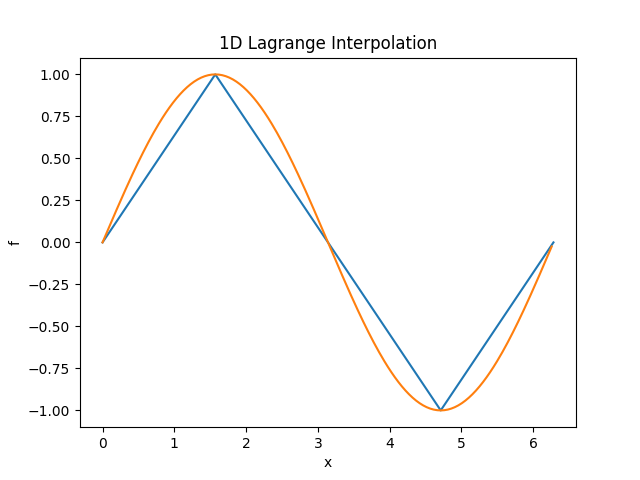
\includegraphics[width=\linewidth]{ex_1D_LG.png}
  \caption{4 Element First Order Interpolation Example and Comparaison to True Solution}
\end{figure}
\\
It follows that we first cut up our domain into a mesh. Commonly these meshes are made up of triangles for simplicity, although squares or even curved elements for simulations on a sphere are also used. Then we approximate $u$ and $p$ using the lagrange element. Hence we get that for instance $u$ is the sum of a set of known piecewise linear functions (as they are determined by the mesh) but with unknown coefficients. The aim of the rest of the method is to determine these unknown coefficients.\\
For that end we need to find what is called the weak form of the equation. We multiply (3) by an arbitrary function $v$. Hence we get :
\begin{align*}
\int_{\omega} -v \cdot \nabla p + \mu v \cdot \nabla^2 u dx = -\int_{\omega} v \cdot F dx
\end{align*}
Since our domain $\omega$ is cut out into triangles we can cut the integral into triangles and work on each one individually. Hence for each cell $e$ in $\omega$ we get : 
\begin{align*}
\int_{e} p \nabla \cdot v + \mu v \cdot \nabla^2 u dx =  -\int_{e} v \cdot F dx
\end{align*}
However since $u$ and $v$ will be approximated by functions which may be discontinuous in their derivatives $\nabla^2$ may not be defined. Hence we need to use integration by parts to get :  
\begin{align*}
\int_{e} p \nabla \cdot v - \mu \nabla v \cdot \nabla u dx = -\int_{e} v \cdot F dx
\end{align*}
Finally multiplying (4) by a similar pressure test function $q$ and adding it to the left hand side of the above we get :
\begin{align}
\int_{e} p \nabla \cdot v - \mu \nabla v \cdot \nabla u dx + \int_{e} q \nabla \cdot u dx = -\int_{e} v \cdot F dx
\end{align}
Now we use the fact that $q$, $v$, $F$, $u$ and $p$ are a sum of known linear functions and coefficients.\\
Pulling out and removing the coefficients of $v$ we get that :
\begin{align*}
 \int_{e} \sum_i \sum_j (  p_j \phi_j \nabla  \cdot \Phi_i - \mu \nabla \Phi_i \cdot u_j \nabla \Phi_j +   \phi_i u_j \nabla \Phi_j) dx = -\int_{e} \sum_i \phi_i F_i \phi_i dx
\end{align*}
Combining all the triangles we can eventually turn our problem into a matrix equation of the form :
\begin{align}
M x = b
\end{align}
Where x is a vector of coefficients of $u$ and $p$.\\
We can solve this using a variety of linear systems solvers. Note in particular that since the majority of basis functions $\Phi$ and $\phi$ are $0$ in any given triangle the matrix $M$ will be sparse.\\
While we locally enforced the divergence-free equation by including it in the weak form, the global flow may not be divergence-free. In order to achieve that more complex mathematical tools would be required.\\
Now apply this to the manufactured solution :
\begin{align*}
u_x &=  -sin(2 \pi y) cos(2 \pi y)  sin(2 \pi x)^2 \\
u_y &= sin(2 \pi x) cos(2 \pi x)  sin(2 \pi y)^2 \\
p &= sin(2 \pi x)^2 sin(2 \pi y)^2 \\
F &= \nabla p - \mu \nabla^2 u
\end{align*}
Where $F$ was selected specifically to ensure that any given $u$ and $p$ are solutions.
Using the above and implementing it in firedrake we get figures .On a mesh with vertices we get an error of about.\\
However default implementation using the CG method is slow, hence we wish to improve on it.

\section{Tools and Definitions}
\subsection{Brezzi-Douglas-Marini Element}
The paper Common and Unusual Finite Elements [7] states that the BDM space on one triangle $K$ is composed by polynomials of order $q$ defined by the normal component on each edge. If $q > 1$ it is also defined using the integration against gradients of the polynomials on the triangle. If $q > 2$ we then also use the integration  against curls of $b_K P_{q-2}(K)$ where $b_{q-2}$ is the  cubic bubble function associated with $K$ and $P_{q}(K)$ is the set of polynomials defined on $K$.\\
This finite element, combined with the DG element for pressure, discretizes the function space H(div). A property we thus get from simply working in BDM is that our solution will be exactly divergence free globally and locally.
Additionally we will be able to employ an enhanced lagrangian preconditioner thanks to the global divergence free property [2].\\

However unlike the lagrange elements we can no longer set a dirichelet boundary condition's tangential component. Therefore we need to find alternative approaches to enforce these conditions.
Additionally some operations (such as the weak form of the curl) are undefined in this space. Due to possible discontinuities at the boundaries we have to be carefull with all boundary integrals.\\

In general the weak form will be far more involved.


\subsection{Discontinous Galerkin and BDM-DG Mixed Space}
The discontinous Galerkin Element space is the space of piecewise linear continuous functions. An example applying this space on its own can be found [8].\\
Combined with the BDM space we obtain a mixed finite element space which approximates the $H_{div}$ finite element space.\\

\subsection{Newton's Method}

Newton's method is a generalized method for solving non-linear matrix equations of the form :
$$
F(x,y) = 0
$$
Where $F$ is a vector function and $x$ is vector of unknowns. Note that $F$ may be non-linear and have constant components.
For instance we could have $ F = x^T A x + M x - b$, where A and M are constant matrices and b is a constant vector.\\ 
We start with a guess $x = x_0$ and then determine the Jacobian of $F(x)$, call it $DF(x)$.\\
We determine the jacobian by calculating the Gateaux derivative, defined as follows [12] :
\begin{align}
DF_{x_n}(\Delta x) = lim_{t \rightarrow 0^+} \frac{F(x_n+ \epsilon \Delta x) - F(x_n)}{\epsilon}
\end{align}
We then use the vector taylor expansion :
\begin{align*}
F(x_{n+1}) = F(x_n) + DF_{x_n}(\Delta x) \Delta x 
\end{align*}
Hence we get the algorithm :
\begin{align}
DF_{x_n}(\Delta x) \Delta x = - F(x_n)\\
x_{n+1} = x_n + \Delta x 
\end{align}
We solve for $\Delta x$ using $x_n$ and the taylor expansion approximation and then use this result to determine $x_{n+1}$.
This is a linear problem which can be solved via an Lu Factorization for instance.\\
Note that the Newton's method only converges and is unique if it is within a ball around the solution [10-11].

\subsection{Preconditioners}

We will first describe how preconditioners, such as the Schur Preconditioner work in general. We see this in the book Multilevel Block Factorization Preconditioners [4] on pages 49 to 51.\\
Take the system :\\
$$
Mx = b
$$
Where $M$ is a very large matrix, assumed for simplicity to be symmetric, $x$ and unknown vector we need to solve for (in our case this will be a vector of coefficients for both $u$ and $p$) and $b$ a constant vector. If $M$ is a symmetric positive definite sparse matrix then $M$ applied to a vector is cheap to compute. Hence we can easily find $r$ the residual such that :\\
$$
r = b - Mx
$$
We then use the resulting $r$ in order to provide a correction on our result.\\
However $M$ may not be well-behaved. In fact in our problem we know it is usually not.\\
In this case we use a preconditioning matrix, $P$ to map the system in such a way that $P^{-1}$ is cheap to compute, this operation can easily be parallelized and the condition number, the ratio of largest and smallest eigenvalue which describes the behaviour of the system [13], is lowered.
We then numerically solve the transformed and hopefully better behaved system : 
$$
P^{-1}(Mx-b) = 0
$$ 

\subsection{Notation}

Regarding the meaning of $a_+$ and $a_-$.\\
When the mesh is setup the software ensures each facette (ie edge of a triangle) in the mesh has a positive and negative side, and each cell agrees on which is which. We call this term on facette integrals, as otherwise it has no meaning. Then $a_+$ is the value of $a$ on the positive side $a_-$ on the negative side.\\
It is important to note that the positive and negative side are completly arbitrary. They serve as markers for the software.\\
For facettes which are facing the exterior domain the normal is always pointing outwards.\\
\\
Let $\{ a \} = a_+ + a_-$. \\
This is an average term. Due to discontinuities of our space on facette elements integrals over facets from integration by parts on an individual element will not dissappear necessarily, hence these terms remain. Additionally, since we cannot use dirichelet boundary conditions, weak penalty terms will also use this operation.\\

For integrals over outer facettes we explicitly write out the formula for clarity.\\
\\
Similarly let $J(a) = a_+ - a_-$\\
This is a jump term. Note that this operation is $0$ in continuous space, which is where we assume the physical fluid velocity and pressure to be.\\
\\
We may have surface integrals over interior facettes and exterior facettes, which are on the computational boundaries.\\
In the first case the integral of $a$ is $\int_\Gamma a dS$ while in the latter we note $\int_{\delta \Omega} a ds$.\\
This is used both for additional clarity and because it is the notation in the code.\\
\\
sgn(k) is the sign of scalar k.


\section{Implementing the $H_{div}$ Solver}
Since we have two problem terms we will deal with each separately. Hence we will first consider the stokes equation, ignoring the advection term and focusing on the viscosity term for now :
\begin{align}
0 &= -\nabla p + \mu \nabla^2 u + F  \\
\nabla \cdot u &= 0
\end{align}

\subsection{Stokes Equation}
We start off by cutting our computational domain $\Omega$ into a set of cells $e$. As discussed above it is now required to find the weak form of equations (9) and (10).
For this purpose let us introduce two test functions, $w$ in BDM for velocity and $q$ in DG for pressure.
Let us multiply equation (9) by $v$ and integrate over the domain as seen in the first section.
\begin{align*}
\int_\Omega v \cdot F dx &= \int_\Omega (v \cdot \nabla p) dx - \int_\Omega (\mu v \cdot \nabla^2 u) dx
\end{align*}

Again we can work on each cell $e$ individually and them sum it all up, hence get :
\begin{align*}
\sum_e \int_e v \cdot F dx &= \sum_e (\int_e (v \cdot \nabla p) dx - \int_e (\mu v \cdot \nabla^2 u) dx)
\end{align*}
Focusing on the viscosity, or second, term we get via integration by parts :
\begin{align*}
\int_e (v \cdot \nabla^2 u) dx = - \int_e \nabla_h(v) : \nabla_h(u) dx + \int_\Gamma 2 \{ v_i n_j \} \{ \frac{\partial u_i}{\partial x_j}\} dS
\end{align*}
The first term can be summed up to an integral over $\Omega$ and the second one is asymmetrical. We can add a term to make it symetrical. This helps with numerical stability of the final matrix equation. Numerical stability ensures that if there are errors in the input values of the problem (such as the exact values of an inflow), they lessen as the algorithm progresses. This property is obviously desirable especially when considering experimental information. Additionally some linear solvers take advantage of this structure.\\
Hence this term becomes :
\begin{align*}
-  \int_\Omega \nabla_h(v) : \nabla_h(u) dx + \sum_e( \int_\Gamma 2 \{ v_i n_j \} \{ \frac{\partial u_i}{\partial x_j}\} dS + \int_\Gamma 2 \{ u_i n_j \} \{ \frac{\partial v_i}{\partial x_j}\} dS)
\end{align*}
$u$ should be continous in the physical space thus the added term will be $0$ in continuous space. Hence this does not change the equation in physical space.\\
\\
Now we also add the term $\alpha \int_\Gamma \frac{1}{h}  J(v_i) J(u_i) dS$. According to sources [3] provided that  $\alpha$ is larger than $10$ numerical stability is increased.\\
$J$ is the jump notation.\\
The numerical value of $h$ is the average distance of a side. In our case we defined it as the average cell-volume over the length of the facettes between them for each individual facette element $\Gamma$.\\
The $J(u_i)$ term makes this integral $0$ in continous space so this does not change the solution.\\
\\
As mentioned in the BDM definition section we cannot set the tangential component of a dirichelet boundary condition in the conventional finite element manner.  So instead we use penalty terms, which should be $0$. This pushes the solution towards respecting the boundary conditions. In practice this just means taking all the terms over the edge of a cell and considering them on the sections of the edge of the domain where dirichelet conditions apply instead.\\
 Hence our final viscous term becomes :\\
\begin{align*}
&-  \int_\Omega \nabla_h(v) : \nabla_h(u) dx + \sum_e ( \int_\Gamma 2 \{ v_i n_j \} \{ \frac{\partial u_i}{\partial x_j}\} dS + \int_\Gamma 2 \{ u_i n_j \} \{ \frac{\partial v_i}{\partial x_j}\} dS \\
&- \alpha \int_\Gamma \frac{1}{h}  J(v_i) J(u_i) dS \ ) + \int_{\partial  \Omega} v_i n_j \frac{\partial(u_i + u^0_i)}{\partial x_j} + (u_i + u^0_i) n_j\frac{\partial v_i}{\partial x_j} ds - \alpha \int_{\partial \Omega} \frac{1}{h} v_i(u_i-u^0_i)ds
\end{align*}
Where $u^0_i$ are the boundary values.
We will call this term $\eta_\mu$.\\
Back to our original equation we get : 
\begin{align}
\int_\Omega v \cdot F dx &= \int_\Omega v \cdot \nabla p dx - \eta_\mu
\end{align}
Let us consider the continuity equation again :
\begin{align*}
\nabla \cdot u = 0
\end{align*}
Multiplying by $q$ and integrating we get :
\begin{align*}
\int_\Omega q \nabla \cdot u dx = 0
\end{align*}
This is $0$, so we add this to the weak formulation $(3)$ we obtained, getting one weak formulation which includes both pressure and velocity while also keeping symmetry. \\
We need this since we want to turn the entire system into a single matrix equation which includes all the conditions.\\
Integrating by parts the pressure term get :
\begin{align}
\int_\Omega v \cdot F dx &= \int_\Omega p \ v \cdot n ds - \int_\Omega  p ( \nabla \cdot v) dx + \int_\Omega q (\nabla \cdot u) dx  - \eta_\mu
\end{align}
But v is $0$ on all the boundaries, hence get :
\begin{align}
\int_\Omega v \cdot F dx &= - \int_\Omega  p ( \nabla \cdot v) dx + \int_\Omega q (\nabla \cdot u) dx  - \eta_\mu
\end{align}

\subsection{Applying the Schur Preconditioner to our problem}
In an effort to get our iteration count to be independent of mesh-size, we will apply a Schur preconditioner similarly described in chapter 3 of Multilevel Block Factorization Preconditioners [4] as well as in source [2].\\
This is a well-known method, however as we will be modifying it, we will quickly describe it as well.
Our sytem effectively amounts to solving a matrix equation of the form :
$$ 
\begin{bmatrix} 
A         & B^{T}\\
B         & 0 \\
\end{bmatrix}
\begin{bmatrix} 
u    \\
p     \\  
\end{bmatrix}
=
\begin{bmatrix} 
b    \\
0     \\  
\end{bmatrix}
$$
Where $B$ is the discretized divergence operator and $B^T$ the discrete gradient operator. $A$ contains the viscous term.
Setting $S = - B A^{-1} B^{T}$, we can factorize the above and get an expression whose inverse is : 
$$
\begin{bmatrix} 
I         & - A^{-1} B^{T}\\
0         & I \\
\end{bmatrix}
\begin{bmatrix} 
A^{-1}   & 0\\
0       & S^{-1} \\
\end{bmatrix}
\begin{bmatrix} 
I & 0\\
 - B A^{-1}       & I \\
\end{bmatrix}
$$
Hence, if we can find $A^{-1}$ and $S^{-1}$ we can easily solve the equation. We solve both via a Lu factorization.\\
We solve for $A^{-1}$, or to be exact the operation $A^{-1}v$ via an Lu Factorization. The Lu factorization is a direct solver, and thus is innefficient. The algorithm would have to be performed in a sequential manner, preventing usage of parallelisation. We did mitigate this through the usage of the "mumps" sub-routine. Additionally there was an  However more efficient implementations would require this to be modified.\\
 However $S^{-1}$, the inverse of the shur complement is difficult to determine because it is usually dense. However research has shown [2 \& 9] that we can solve this issue by using a "grad-div" stabilization method. We add the term $\gamma \nabla \cdot v \: \nabla \cdot w$ to the equation (!). Note that this term is 0 in continuous space. We thus get : 
\begin{align}
\int_\Omega w \cdot F dx &= \int_\Omega \nabla \cdot (p v) dx - \int_\Omega ( p \nabla \cdot (v)) dx - \int_\Omega q (\nabla \cdot u) dx  - \eta_\mu + \int_\Omega \gamma \nabla \cdot u \: \nabla \cdot v dx
\end{align}
This doesn't change the equation, thus should result in the same solution. However according to the same papers [2 \& 9] we can then approximate $S$ by the pressure mass matrix. We then perform ILu in order to solve for $S^{-1}$. ILu performs the Lu Factorization on various blocks of the matrix, allowing it to be parallelised.\\
Note that in theory we could have tried a similar method in the CG space.
Testing shows however that this fails.
This makes sense as we utilized the exact divergence free-property of our space for the Schur complement.
As a result in the CG space as gamma tends to infinity S does not exactly tend to the pressure mass matrix.

\section{Full Navier Stokes}
Now we include the advection term : 
\begin{align*}
(u \cdot \nabla) u &= -\nabla p + \mu \nabla^2 u + F
\end{align*}
Note that this is equation is not linear, hence we will need to use Newton's method.\\ 

\subsection{Advection Weak Form}
In order to solve the equation regardless of the method, we need to find the weak form of the advection term, $(u \cdot \nabla) u$.
Similarly to before we therefore take the inner product of the advection term with $q$ and integrate over the domain.
\begin{align}
\int_\Omega (u \cdot \nabla)u \cdot v \ dx
\end{align}
Consider the following vector identity :
\begin{align*}
\nabla (u \cdot u) = 2 (u \cdot \nabla) u + 2 u \times (\nabla \times u) 
\end{align*}
Hence get : 
\begin{align}
\int_\Omega (u \cdot \nabla)u \cdot v \ dx = \frac{1}{2} \int_\Omega \nabla (u^2) \cdot v \ dx - \int_{\Omega} u \times (\nabla \times u) \cdot v \ dx
\end{align}
We can then perform an integration by parts on the first term on the right hand side to get :
\begin{align}
 \frac{1}{2} \int_\Omega \nabla (u^2) \cdot v \ dx = \frac{1}{2} (\int_{\delta \Omega } u^2 v \cdot n \ ds - \int_\Omega u^2 \nabla \cdot v \ dx)
\end{align}
Now consider the second term in (17)
\begin{align*}
- \int_{\Omega} u \times (\nabla \times u) \cdot v \ dx &= \int_{\Omega} v \cdot (\nabla \times u) u \ dx   \\
&=  \int_{\Omega} (\nabla \times u) \cdot (u \times v)  \ dx
\end{align*}
Next we use the results from source [?].\\
From this we obtain that via integration by parts on each individual element we get : 
\begin{align*}
\sum_e \int_e u \cdot (\nabla \times (u \times v) \ ) dx - \int_{\Gamma} \frac{1}{2}(\{u\} + sgn(u \cdot n)[u]) \cdot (n \times (u \cdot v) \ ) dS
\end{align*}
Hence get :
\begin{align}
&\int_\Omega u \cdot (\nabla \times (u \times v) \ ) dx -  \sum_e \int_{\Gamma} u_{up} \cdot (n \times (u \cdot v) \ ) dS \\
& u_{up} = \frac{1}{2}((sgn(u \cdot n) + 1)_+ u_+ + (sgn (u \cdot n) +1)_- u_-)
\end{align}
$u_{up}$ is the upwinding term mentioned in the paper.\\
Note that it is equal to $u^+$ if $n$ is in the "positive" direction, and $u^-$ otherwise. (Reminder : the positive and negative direction are arbitrarily set when creating the mesh. They serve solely as markers for the software)\\
Note that the second term becomes the following on the computational domain boundary :
\begin{align*}
- \int_{\delta \Omega} u_0 \cdot (n \times (u \cdot v) \ ) ds
\end{align*}
Hence the weak form of our advection term is : 
\begin{align}
 Adv &= \int_\Omega u \cdot (\nabla \times (u \times v) \ ) dx - \int_{\Gamma} u_{up} \cdot (n \times (u \cdot v) \ ) dS \\ 
&- \frac{1}{2} \int_\Omega u^2 \nabla \cdot v \ dx - \int_{\delta \Omega} u_0 \cdot (n \times (u \cdot v) \ ) ds
+ \frac{1}{2} \int_{\delta \Omega } u^2 v \cdot n \ ds 
\end{align}
We reordered some terms to be in-line with our code.

\subsection{Continuation Method}

Given the navier stokes equations we could try to naively solve directly applying the above preconditioning and discretization methods. However at high Reynolds number this approach quickly fails unless the mesh is refined or a better initial guess is given, leading to high computational cost.\\
Hence consider the modified equation :
\begin{align}
c (u \cdot \nabla) u &= -\nabla p + \mu \nabla^2 u + F
\end{align}
As mentioned in the Newton's Method section, the Newton's Method converges only if the initial guess is within a certain ball around the solution. Hence we need to find a method to get our initial guess to be closer to the solution.\\
We could use the stokes solution as an initial guess, which we can most likely solve. We then increase $c$ to $1$ and try to solve using the stokes solution as a guess. \\
If it still fails we can take $c =0.5$ before solving for full advection. If necessary we can bring downthe value of $c$ multiple times until our solver converges at an appropriate rate. Afterwards we then gradually increase c using the same procedure until we solve for full advection.\\
\\
We can speed up this process in two ways.\\
The first, very simple method, is adapting our step-size to the problem. Rather than starting with a step size of $1$ we can reduce the step size initially if the Reynolds number is high enough. In addition to reducing the stepsize if the newton iteration fails, we can increase step size if it succeeds. This should allow us to close in on the optimal step size rapidly. This allows us to reduce the total number of times we try to use the Newton's method.\\
The second involves approximating the $(u,p)$ at a subsequent step more accuratly. Rather than just using the prior value of $(u,p)$, call it $x_c$, we use taylor expansion. We can consider $x_c$ to be a function of $c$, hence get :
$$
x_{c+\Delta c} = x_c + \Delta c \frac{\partial x_c}{\partial c}
$$
Provided we can find $\frac{\partial x_c}{\partial c}$ this will give us a far more accurate solution.
To find the derivative of $x_c$ with respect to $c$ we consider :\\

Which we sp;ve via a newton iteration.\\
In some circumstances however even with a variable step-size in $c$ we fail to obtain a solution within an acceptable time-frame. In our code if the step-size is below $10^{-3}$ our solver stops and fails. This usually happens for high Reynaulds number flows.

\section{Stability Analysis}

While we are mainly interested in the steady-state solution of the navier-stokes equation we also need to consider whether or not the solution is stable. To that end we need to solve a full navier stokes, including the time derivative. This will be used to determine if small perturbations of the solution die down.
\subsection{Time stepping method}
In practice our problem amounts to the following, very generalized, equation : 
\begin{align}
F(u) = 0
\end{align}
Where F is some function. this is in practice how the firedrake non-linear solver solves the equation.\\
If we add in the time-terms we get :
\begin{align}
\frac{\partial u}{\partial t} + F(u,p) = 0
\end{align}
While we could try and solve this equation directly using Backwards Euler or Midpoint Rule testing shows that this does not converge. Instead we use Picards iteration along with the Midpoint rule as described in the following equation :
\begin{align}
u^{n+1} - u^n + \Delta t (\frac{1}{2}G(u^n,p^n) + \frac{1}{2} G(u^{n+1},p^{n+1}) + ( u^n \cdot \nabla u^n) ) = 0
\end{align}
Here $G = RHS - LHS $. We applied the midpoint rule to the linear terms of the equation while the non-linear term, the advection term, was evaluated at the previous time step. Provided the time step is low enough this will always converge, regardless of inital guess.
Optionally we could afterwards use the method we described first, Newton's method and Midpoint Rule, to get a more accurate result after a few Picards iterations.
\begin{align}
u^{n+1} - u^n + \Delta t (\frac{1}{2}F(u^n,p^n) + \frac{1}{2} F(u^{n+1},p^{n+1})) = 0
\end{align}

\subsection{Perturbation}

When interested in the stability of a solution analytically we commonly first determine the solution. We would then consider the normal modes form of the equation before perturbing it. After some algebra we determine the most unstable mode and deduce from that.\\
While there are methods to determine these unstable modes numerically we will not use either of these methods here.\\
Instead we will use a far simpler algorithm.
We will consider random perturbations and then use the time stepping method to see if they grow.

\section{Test Cases}
\subsection{Stokes Convergence}

Once again we will primarily focus on the stokes equation (9-10) in order to verify that this part of our discretization is working as intended.\\
We will consider a manufactured solution, an artificial solution we selected in advance. Take $u_x = sin(2 \pi y) cos(2 \pi y)*sin(2 \pi x)^2$, $u_y= -sin(2 \pi x) cos(2 \pi x) sin(2 \pi y)^2$ and $p = sin(2 \pi x) sin(2 \pi y)$.\\
We then adjust the boundary conditions and forcing term appropriately for this solution to hold.\\
 The forcing term thus becomes :$F = \nabla p - \mu \nabla^2 u$.\\
Figures and show us the convergence graphs in velocity and pressure.\\
This shows that the preconditioning and discretisation holds as expected for the stokes equation if boundary conditions are $0$.
\\

\begin{figure}
  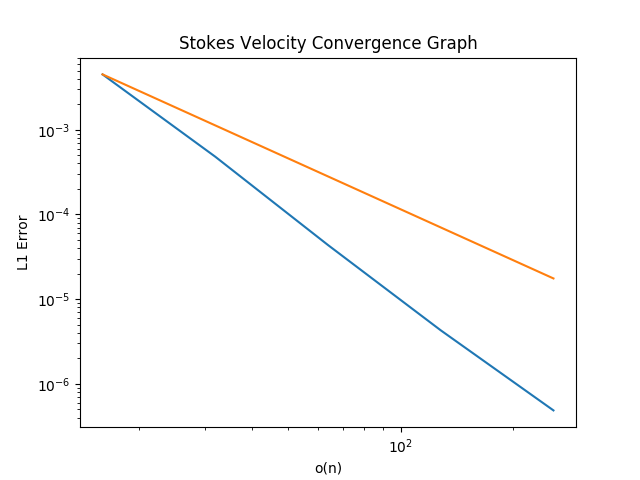
\includegraphics[width=\linewidth]{stokes_convergence_dbc0.png}
  \caption{DG2-BDM1 Stokes velocity Convergence Graph. As expected the velocity error has an order 2 convergence}
\end{figure}

\begin{figure}
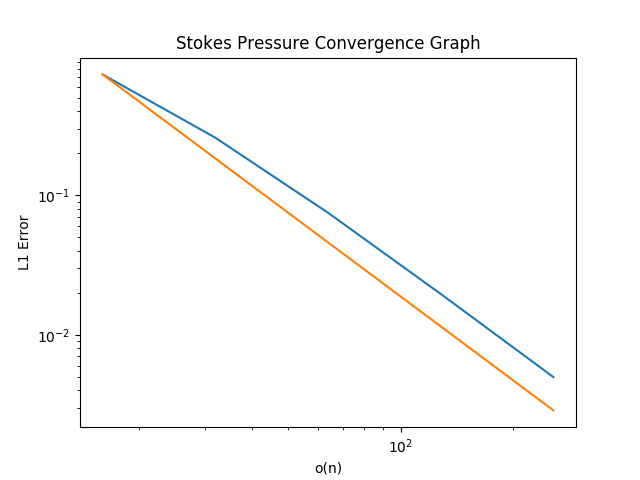
\includegraphics[width=\linewidth]{stokes_pressure_convergence_dbc0.png}
  \caption{DG2-BDM1 Stokes velocity Convergence Grap. As expected the pressure error has an order 2 convergence}
\end{figure}

\subsection{Navier-Stokes Convergence}

We again use a manufactured solution to determine the convergence rate of our solver.
We can re-use the first solution in the stokes convergence test, $u_x = sin(2 \pi y) cos(2 \pi y)sin(2 \pi x)^2$, $u_y= -sin(2 \pi x) cos(2 \pi x) sin(2 \pi y)^2$ and $p = sin(2 \pi x) sin(2 \pi y)$.\\
However the forcing term will now be $F = \nabla p - \mu \nabla^2 u + u \cdot \nabla u$.
Plugging this into the equations we get that these do indeed solve the navier-stokes equations.\\
Figures and show us the convergence graphs in velocity and pressure.\\

\begin{figure}
  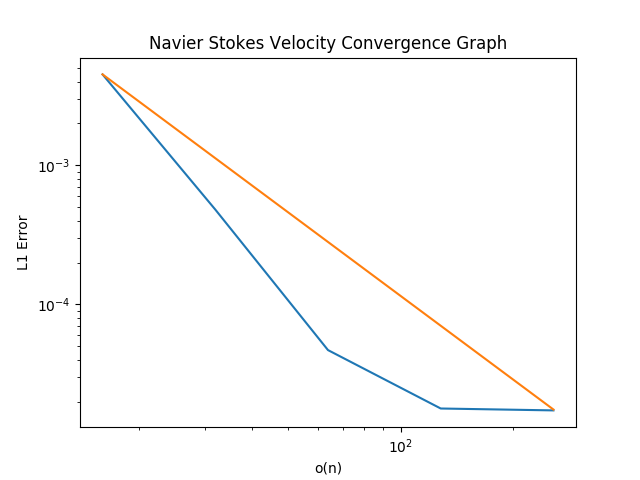
\includegraphics[width=\linewidth]{navier_stokes_convergence_dbc0.png}
  \caption{DG2-BDM1 Navier Stokes velocity Convergence Graph. As expected the velocity error has an order 2 convergence}
\end{figure}

\begin{figure}
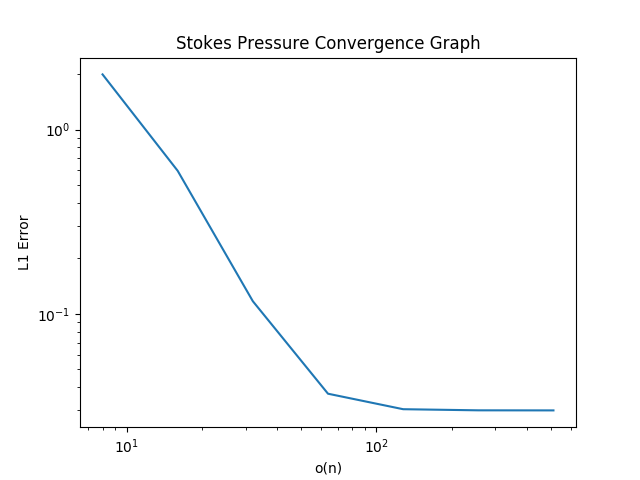
\includegraphics[width=\linewidth]{navier_stokes_pressure_convergence_dbc0.png}
  \caption{DG2-BDM1 Navier Stokes velocity Convergence Grap. As expected the pressure error has an order 2 convergence}
\end{figure}

Note that we did not reuse the manufactured solution from the stokes convergence test for non-zero boundary conditions, as a matter of fact applying those we get figures and  for velocity and pressure. These show non-convergence, which is confirmed when considering the error graph in space in figure.\\
While this might have indicated some error in the solver it turns out this is to be expected. In this scenario the equation is ill-posed. The exact reason is unkown, as this is still an active field of research. However a rule of thumb is that if you have dirichelet outflow the equation is ill-posed. An intuitive way of explaining this is that if we were to expand our domain the out of bounds flow might still be able to affect the flow in the computational domain (for instance trailing vorticies) in ways that we would thus not be able to capture if this region was excluded. 

\subsection{Known Case : Flow between concentric circles}

We will study this relatively simple problem as means to demonstrate the ability of our solver to work even on non-uniform arbitrary meshes and solve an unsteady problem.\\
The problem takes place in the annulus between two concentric circles each rotating at a different speed. For our steady case we will consider unit circle rotating at speed $1$ and circle of radius $2$ rotating at speed $3$. 
From [16] we get that the general solution of the tangential velocity and pressure for this problem is of the form :
\begin{align}
u_{\phi} = C_1 r + \frac{C_2}{r} \\
p = \rho \int \frac{u_{\phi}^2}{r} dr + C
\end{align}
From the above boundary conditions are $u_{\phi}(r=1) = 1$, $u_{\phi}(r=2) = 3$. Hence get :
\begin{align*}
C_1 = 1 - C_2 
\end{align*}
Figures show pressure and velocity in this case.\\

Now consider the outer circle initially immobile, but slowly accelerating until it reaches tangential speed of $3$. The velocity solution at different time steps is shown in figures.

\subsection{Known Case : Flow Past a Cylinder}

The flow past a cylinder is a well-known and studied flow with interesting properties, namely in stability of its steady solution.\\
Hence we will see how our solver resolves this flow and compare results with other papers [14].

\subsection{Known Case : Cylinder flow Stability}

\section{Conclusion and Future Improvements}

In this project we were interested in applications of the BDM/DG mixed finite element onto the steady navier-stokes equations.\\
After briefly discussing the general finite element method and some introductory definitions and notations we descided to focus on the stokes equation. After assembling the weak form of the equation we then applied a Schur preconditioner to  improve efficiency.\\
We then assembled a weak form of the Navier-Stokes equation but noted that directly using it wasn't optimal. As such we developed a continuation method with variable step-size to improve the algorithm's speed and expand the number of problems which it can solve.\\
After this we made a rudimentary time-stepping method to study the stability of any solutions obtained.\\
Finally we tested all of the above and concluded that our algorithm worked as anticipated.\\
\\
\\
However a number of future improvements could be made.\\
\\
We could use a multigrid method using our method as a smoother to get convergence to be less dependent on grid-size, dramatically reducing computational costs. Application of such a method was discussed, unfortunatly the tools required for it are not currently compatible with our problem set (specifically dirichelet boundary conditions).\\
The variable step-size method is servicable but can be considerably improved to reduce the total number of iterations and thus computational cost. There are a number of methods which from local conditions of the function could more efficiently determine an appropriate step-size. Our source on the continuation method [17] includes such improvements.\\
Similarly the time-stepping method was designed exclusively for the stability test. For this purpose it works very well. However various improvements could be made for accuracy and speed. For instance we initially attempted to utilise a Newton iteration rather than a Picards iteration. However as the initial guess wasn't in the ball of convergence this method failed. Adding a few Newton iterations using the picards results as a starting point should give more accurate answers for time-dependent methods.\\
Additionally the stability itself could be expanded to for instance consider the growth rate of an instability as well as determines unstable modes.\\
In some flows we may have multiple solutions or a bifurcation (that is the case for the cylinder flow at high Reynolds number). In this case a deflation method may be usefull. In this method, after finding a solution we "substract" it from the equation and thus seek other solutions.

\section{Appendix}
\subsection{Discussing the Code}
A significant part of this project was developing a python code using firedrake.
Firedrake is a python project which aims to provide mathematicians, engineers and scientists with an automated system for solving partial differential equations.\\
It does so by automatically generating code based on UFL expressions from the fenics project, a library of computational methods used for solving PDEs. This allows us to write out our equations in a fairly intuitive way while firedrake generates the background code needed to solve them.\\
Our project comprises largely of one file containg the rinsp and rinspt classes, though various launching scripts and the lagrange script are also present. We will not discuss the entirety of either class, if the reader wants to have a detailed look he can go to the github repository containg it at https://github.com/Frostyant/M4R\_Navier\_Stokes\_Solvers once it has been made public.\\
We will however show a handfull of code snippets, ranging from the parameters firedrake uses to the generate the code to the ufl expressions for the viscous, pressure and advection terms.

\subsubsection{Solver Paremeters}
The parameters of our solver are :
\begin{lstlisting}
"ksp_type": "gmres",
            "ksp_converged_reason": True,
            "ksp_rtol": 1e-6,
            "ksp_max_it": 50,
            "pc_type": "fieldsplit",
            "pc_fieldsplit_type": "schur", #use Schur preconditioner
            "pc_fieldsplit_schur_fact_type": "full", #full preconditioner
            "pc_fieldsplit_off_diag_use_amat": True,
            "fieldsplit_0_ksp_type": "preonly",
            "fieldsplit_0_pc_type": "lu",#use full LU factorization, ilu fails
            "fieldsplit_0_pc_factor_mat_solver_type": "mumps",
            "fieldsplit_1_ksp_type": "preonly",
            "fieldsplit_1_pc_type": "bjacobi",
            "fieldsplit_1_pc_sub_type": "ilu"#use incomplete LU factorization on the submatrix
\end{lstlisting}
GMRES indicates the solver used for the outer system.
 It stands for generalized minimal residual method, and used due to nonsymmetric nature of our equation.\\
ksp\_rtol indicates the relative tolerance above which we consider that the equation diverges.\\
ksp\_max\_it is the maximal number of iterations for the linear GMRES solver. If above it the solver fails or, in the continuation method, reduces the advection term and tries again.\\
"pc\_type": "fieldsplit" and "pc\_fieldsplit\_type": "schur" indicates we are using the Schur fieldsplit preconditioner.\\
"fieldsplit\_0 options deal with finding $A^{-1}$ in the Schur Preconditioner wjile the fieldsplit\_1 options deal with the remaining part of the preconditioner.

\subsubsection{Viscous Term}
The code associated to the viscous term is :
\begin{lstlisting}
def GetViscousTerm(self,u,p):
        """Gets Main Viscous Terms
        Keyword arguments:
        u -- velocity
        p -- pressure
        Outputs :
        viscous_term -- RHS Viscous terms (ie they depend on up)
        L -- LHS Viscous Terms (They do not depend on up)
        """
        c = Constant(20)
        n = FacetNormal(self.mesh)
        h = avg(CellVolume(self.mesh))/FacetArea(self.mesh)

        if self.BcIds == False:
            viscous_stab_L = c/(h)*inner(self.v,self.u_0)*ds
            viscous_byparts2_ext_L = 1/2*(
            + inner(outer(self.u_0,n),grad(v))*ds
            + inner(outer(self.v,n),grad(self.u_0))*ds
            )
        else:
            viscous_stab_L = c/(h)*inner(self.v,self.u_0)*ds(self.BcIds)
            viscous_byparts2_ext_L = 1/2*(
            + inner(outer(self.u_0,n),grad(self.v))*ds(self.BcIds)
            + inner(outer(self.v,n),grad(self.u_0))*ds(self.BcIds)
            )

        L = viscous_stab_L + viscous_byparts2_ext_L

        #Viscous Term parts
        viscous_byparts1 = inner(grad(u), grad(self.v))*dx #this is the term over omega from the integration by parts
        viscous_byparts2 = 2*inner(avg(outer(self.v,n)),avg(grad(u)))*dS #this the term over interior surfaces from integration by parts
        viscous_symetry = 2*inner(avg(outer(u,n)),avg(grad(self.v)))*dS #this the term ensures symetry while not changing the continuous equation
        viscous_stab = c*1/(h)*inner(jump(self.v),jump(u))*dS #stabilizes the equation
        if self.BcIds == False:
            viscous_byparts2_ext = 1/2*(inner(outer(self.v,n),grad(u)) + inner(outer(u,n),grad(self.v)))*ds #This deals with boundaries
            viscous_ext =c/(h)*inner(self.v,u)*ds#this is a penalty term for the boundaries
        else:
            viscous_byparts2_ext = 1/2*(inner(outer(self.v,n),grad(u)) + inner(outer(u,n),grad(self.v)))*ds(self.BcIds) #This deals with boundaries
            viscous_ext =c/(h)*inner(self.v,u)*ds(self.BcIds)#this is a penalty term for the boundaries
        #Assembling Viscous Term
        viscous_term = self.viscosity*(
            viscous_byparts1
            - viscous_byparts2
            - viscous_symetry
            + viscous_stab
            - viscous_byparts2_ext
            + viscous_ext
        )

        L = self.viscosity*L

        return viscous_term,L
\end{lstlisting}
Note that in case we do not have dirichelet boundary conditions we obviously didn't integrate the exterior term over those boundaries (hence the ds(self.BcIds)).

\subsubsection{Pressure Term}
The code associated to the Pressure and graddiv term is :
\begin{lstlisting}
def GetBilinear(self,u,p,viscous_term):

        #Setting up bilenar form
        graddiv_term = self.gamma*div(self.v)*div(u)*dx
        a_bilinear = (
            viscous_term +
            self.q * div(u) * dx - p * div(self.v) * dx #Pressure terms from second integ by parts
            + graddiv_term
        )
        return a_bilinear,graddiv_term
\end{lstlisting}
Note that we needed to combine the two equations (continuity and momentum) to be able to use the mixed BDM/DG vector space.

\subsubsection{Advection Term}
The code associated to the Advection term is :
\begin{lstlisting}
def GetAdvectionTerm(self,up,InflowBc,Bcs):

        n = FacetNormal(self.mesh)
        #splitting u and p for programming purposes (unavoidable)
        u, p = split(up)

        #Re-Defining functions for use in Advection term
        if self.twoD:
            curl = lambda phi: as_vector([-phi.dx(1), phi.dx(0)])
            cross = lambda u, w: -u[1]*w[0]+u[0]*w[1]
            perp = lambda n, phi: as_vector([n[1]*phi, -n[0]*phi])
        else:
            perp = cross

        #Defining upwind and U_upwind for use in advection
        Upwind = 0.5*(sign(dot(u, n))+1)
        U_upwind = Upwind('+')*u('+') + Upwind('-')*u('-')

        #Assembling Advection Term
        adv_byparts1 = inner(u, curl(cross(u, self.v)))*dx #This is the term from integration by parts of double curl
        adv_byparts2 = inner(U_upwind, 2*avg( perp(n, cross(u, self.v))))*dS #Second term over surface
        adv_grad_parts1 = 0.5*div(self.v)*inner(u,u)*dx #This is the term due to the integration by parts of grad u^2
        if not InflowBc:
            adv_bdc1 = inner(u,perp(n,cross(u,self.v)))*ds(Bcs) #boundary version of adv_byparts2
            adv_grad_parts2 = 1/2*inner(inner(u,u)*self.v,n)*ds(Bcs) #boundary term from grad u^2 integration by parts
        else:
            adv_bdc1 = inner(u,perp(n,cross(u,self.v)))*ds(Bcs) #boundary version of adv_byparts2
            adv_grad_parts2 = 1/2*inner(inner(u,u)*self.v,n)*ds(Bcs) #boundary term from grad u^2 integration by parts
            adv_bdc1 +=  inner(self.u_0,perp(n,cross(self.u_0,self.v)))*ds(InflowBc) #boundary version of adv_byparts2
            adv_grad_parts2 += 1/2*inner(inner(self.u_0,self.u_0)*self.v,n)*ds(InflowBc) #boundary term from grad u^2 integration by parts

        advection_term = (
            adv_byparts1
            - adv_byparts2
            - adv_grad_parts1
            - adv_bdc1
            + adv_grad_parts2
        )

        return advection_term
\end{lstlisting}
Note that inflow boundary conditions have to be treated separatly from no-slip boundary conditions.

\section{Citations}

[1] Imperial College London \textit{Firedrake Project} Available from : https://www.firedrakeproject.org [Accessed througout 2018-2019]\\

[2] Patrick E. Farrell, Lawrence Mitchell, Florian Wechsung
 An Augmented Lagrangian Preconditioner For The 3D Stationary Incompressible Navier–Stokes Equation At High Reynolds Number
\textit{SIAM J. Sci Comput 28(6)}2006\\

[3] Arnold, Douglas N., et al. "Unified analysis of discontinuous Galerkin methods for elliptic problems." SIAM journal on numerical analysis 39.5 (2002): 1749-1779.\\

[4] Vassilevski, Panayot S. Multilevel Block Factorization Preconditioners: Matrix-based Analysis and Algorithms for Solving Finite Element Equations. New York, NY: Springer New York, 2008. Web.\\

[5] Ibrahimbegovic, Adnan. \textit{Nonlinear Solid Mechanics}. Vol. 160. Dordrecht: Springer Netherlands, 2009. Solid Mechanics and Its Applications. Web.\\

[6] Thomée, Vidar. (1986). \textit{Galerkin finite element methods for parabolic problems}. SERBIULA (sistema Librum 2.0). 25. 10.1007/978-3-662-03359-3. \\

[7]  Kirby R.C., Logg A., Rognes M.E., Terrel A.R. (2012) \textit{Common and unusual finite elements}. In: Logg A., Mardal KA., Wells G. (eds) Automated Solution of Differential Equations by the Finite Element Method. Lecture Notes in Computational Science and Engineering, vol 84. Springer, Berlin, Heidelberg\\

[8] Hansbo, Peter \& Larson, Mats. (2003). \textit{Discontinuous Galerkin and the Crouzeix–Raviart element: Application to elasticity}. http://dx.doi.org/10.1051/m2an:2003020. 37. 10.1051/m2an:2003020. \\

[9] Olshanskii, Maxim \& Reusken, Arnold. (2004). \textit{Grad-div stabilization for Stokes equations}. Mathematics of Computation - Math. Comput.. 73. 1699-1718. \\

[10] Huan Zhengda, \textit{The convergence ball of Newton's method and the uniqueness ball of equations under Hölder-type continuous derivatives},
Computers \& Mathematics with Applications,
Volume 47, Issues 2–3,
2004,
Pages 247-251,
ISSN 0898-1221,
https://doi.org/10.1016/S0898-1221(04)90021-1.\\

[11] X Wang, \textit{Convergence of Newton's method and uniqueness of the solution of equations in Banach space}, IMA Journal of Numerical Analysis, Volume 20, Issue 1, January 2000, Pages 123–134, https://doi.org/10.1093/imanum/20.1.123\\

[12] Bae, Jong Sook, and Sangsuk Yie. \textit{Range of Gateaux Differentiable Operators and Local Expansions}  Pacific J. Math. 125.2 (1986): 289-300. Web.\\

[13] Zi-Cai Li, Cheng-Sheng Chien, Hung-Tsai Huang,\textit{
Effective condition number for finite difference method},
Journal of Computational and Applied Mathematics,
Volume 198, Issue 1,
2007,
Pages 208-235,
ISSN 0377-0427,
https://doi.org/10.1016/j.cam.2005.11.037.\\

[14] Hashiguchi, Masanori \& Kuwahara, Kunio. (1996). \textit{Two-Dimensional Study of Flow past a Circular Cylinder}. RIMS Kokyuroku. 974. \\

[15] Cockburn B, Kanschat G, Schötzau D. \textit{A note on discontinuous galerkin divergence-free solutions of the navier-stokes equations. Journal of Scientific Computing}. 2007 Jun 1;31(1-2):61-73. https://doi.org/10.1007/s10915-006-9107-7\\

[16] Constantinescu V.N. (1995) \textit{Other Solutions of Navier-Stokes Equations (Steady Incompressible Flow).} In: Laminar Viscous Flow. Mechanical Engineering Series. Springer, New York, NY

[17] Deuflhard P. (2011) Parameter Dependent Systems: Continuation Methods. In: \textit{Newton Methods for Nonlinear Problems}. Springer Series in Computational Mathematics, vol 35. Springer, Berlin, Heidelberg


\end{document}